\chapter{Caso de Teste}

\section{Apresentação do Sistema}

Para ilustrar o funcionamento do sistema supervisório, foi utilizado um Arduino UNO que simulasse o funcionamento de um processo com dois tanques de área variável acoplados. A Figura \ref{img_sistema_teste} o esquematiza:

\begin{figure}[htb]
	\centering
	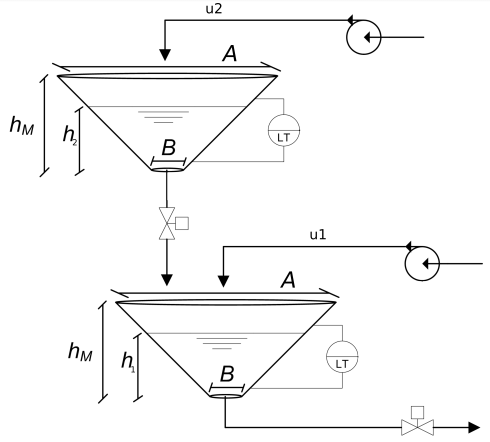
\includegraphics[width=0.8\textwidth,height=0.4\textheight]{sistema_teste}
	\caption{Esquema de leitura serial no supervisório didático\\Fonte: Elaborado pelo Prof. Daniel Santana}
	\label{img_sistema_teste}
\end{figure}

Como percebido pela Figura \ref{img_sistema_teste}, os tanques têm o formato de tronco de cone e as variáveis controladas são suas alturas. A variável de controle são as vazões de entrada de fluido em ambos os tanques.

As equações deste processo são descritas por
\begin{equation}
\frac{dh_1}{dt} = \frac{1}{\beta(h_1)}(u_1 - k\sqrt{\rho g h_1} + k\sqrt{\rho g h_2})\\
\frac{dh_2}{dt} = \frac{1}{\beta(h_2)}(u_2 - k\sqrt{\rho g h_2})\\
\beta(h_i) = \frac{dV}{dh_i}\\
V(h_i) = \frac{\pi\gamma^2}{3}(h_i + \frac{B}{2\gamma})^3 - \frac{\pi}{3\gamma}(\frac{B}{2})^3\\
\gamma = \frac{A-B}{2h_M}\\
\end{equation}
e seus parâmetros e variáveis são descritos e dimensionados na tabela \ref{tbl_parameters}:

\begin{table}[htb]
	\centering
	\begin{tabular} {|m{5em} m{15em} m{8em}|}
		\hline
		Símbolo & Descrição & Valor (u.m.) \\
		\hline
		A & diâmetro superior & 4 ($m$) \\
		B & diâmetro inferior & 1 ($m$) \\
		hm & altura máxima & 4 ($m$) \\
		V & volume & - ($m^3$) \\
		h & altura & - (m) \\
		$\rho$ & densidade do fluido & 1000 ($kg/m^3$) \\
		g & aceleração da gravidade & 9,8 ($m/s^2$) \\
		k & constante de descarga no tanque & 0,001 (-)\\
		u & vazão da bomba & - ($m^3/s$)\\
		\hline
	\end{tabular}
	\caption{Tabela de parâmetros e variáveis do sistema}
	\label{tbl_parameters}
\end{table}

\section{Comportamento esperado}[\label{comportamento_esperado}]

Por se tratar de um sistema não linear, pouco pode-se dizer de seu comportamento dinâmico, partindo-se somente das esquações. Porém, é possível prever possíveis estados estacionários, onde a taxa de variação dos estados no tempo é nula.

Com as derivadas zeradas nas equções descritivas, tem-se que
\begin{equation}
{h_1}_{ss} = (\frac{{u_1}_{ss}}{k\sqrt{\rho g}} + \sqrt{{h_2}_{ss}})^2
\end{equation}
\begin{equation}
{h_2}_{ss} = \frac{{u_2}_{ss}^2}{k^2 \rho g}
\end{equation}
Como os estados estacionários são reais e finitos, o sistema é dito estável. Nota-se também que, caso a bomba 1 seja desligada, é possível manter as alturas em um ponto diferente de zero somente com a acão da bomba 2, e ambas assumirão os mesmos valores eventualmente (${h_1}_{ss} = {h_2}_{ss}$).

\section{Sintonia do Controlador}

Segundo \cite{Lourenco2007}, não é possível determinar o tipo de controlador a se usar numa determinada aplicação. Idealmente, o controlador mais simples, que satisfaça a "resposta desejada" deve ser ser escolhido. Porém, a escolha depende também das condições de operação do sistema e de performance, como o erro estacionário máximo, e o tempo de estabelecimento permitido.

Mantendo-se neste raciocínio, serão comparados dois controladores distintos neste caso de teste. No primeiro caso, o sistema será linearizado em torno de um ponto de operação e o resultado será utilizado para sintonizar um controlador PID. Em seguida o controlador será acoplado ao sistema. No segundo caso, um controlador mais simples será empregado, o chamado LQR, sintonizado por uma equação matemática, descrita na sua respectiva seção neste documento.

\subsection{Linearização do Sistema}

O processo de linearização de um sistema consiste na aplicação da série de Taylor em suas equações descritivas num determinado ponto de operação:

Aplicando a linearização no sistema de estudo, as novas equações do sistema, em desvio, serão então
\begin{equation}
\frac{dh_1}{dt} = -\big(\frac{d\beta^{-1}(h)}{dh}\bigg|_{{h_1}_{ss}} k\sqrt{\rho g {h_1}_{ss}} + \frac{\beta^-1({h_1}_{ss}) k\sqrt{\rho g}}{2\sqrt{{h_1}_{ss}}}\big)\overline{h_1} + \big(\frac{\beta^-1({h_1}_{ss}) k\sqrt{\rho g}}{2\sqrt{{h_2}_{ss}}}\big)\overline{h_2} +  \beta^{-1}({h_1}_{ss})\overline{u_1}
\end{equation},
\begin{equation}
\frac{dh_2}{dt} = -\big(\frac{d\beta^{-1}(h)}{dh}\bigg|_{{h_2}_{ss}} k\sqrt{\rho g {h_2}_{ss}} + \frac{\beta^-1({h_2}_{ss}) k\sqrt{\rho g}}{2\sqrt{{h_2}_{ss}}}\big)\overline{h_2} + \beta^{-1}({h_1}_{ss})\overline{u_2}
\end{equation}
\begin{equation}
\beta^{-1}(h) = \frac{4}{4\pi(\gamma h)^2 + 4B\gamma h + B^2} 
\end{equation}
\begin{equation}
\frac{d\beta^{-1}(h)}{dh} = -4 \frac{8 \pi \gamma^2 h + 4 \gamma B}{(4\pi(\gamma h)^2 + 4B\gamma h + B^2)^2}
\end{equation}

Substituindos os parâmetros de acordo com a tabela \ref{tbl_parameters} e em formato de espaço de estados o sistema final linearizado será

\begin{equation}
\begin{pmatrix} \dot{\overline{h_1}} \\ \dot{\overline{h_2}} \end{pmatrix} = \begin{pmatrix} -0,063 & 0,046 \\ -0,063 & 0 \end{pmatrix} \begin{pmatrix} \overline{h_1} \\ \overline{h_2} \end{pmatrix} + \begin{pmatrix} 0,937 & 0 \\ 0 & 0,937 \end{pmatrix} \begin{pmatrix} \overline{u_1} \\ \overline{u_2} \end{pmatrix}
\label{espaco_estados}
\end{equation}

\subsection{Sintonia do PI}

O controlador PI é um tipo bastante utilizado na indústria. Possui um ganho proporcional (P) e um ganho integrativo (I), que incidem sobre a diferença entre a medição atual de uma saída de processo e seu valor desejado. Isto exige que o sistema de controle seja realimentado com um valor geralmente advindo de um sensor, constituindo-o num sistema de malha fechada. A sintonia de um PI se traduz na definição de P e I, e pode ser realizada, entre outras formas, por métodos como Ziegler-Nichols, Coher-Coon ou até mesmo tentativa e erro.

\begin{displayquote}
	"Nos métodos práticos de sintonia o primeiro passo na utilização dos controladores standard P, PI, PD, PID tem como principal decisão a escolha dos modos a utilizar (proporcional, derivativo, integral, ou uma combinação destes). Uma vez aquela tomada, procede-se ao ajustamento dos vários parâmetros do controlador. O ajustamento ou calibração do controlador (sintonização de controladores) consiste em deduzir, partindo da resposta do sistema, quando este é sujeito a entradas específicas, determinados valores que vão permitir o cálculo dos referidos parâmetros." \cite{lourenco2007}
\end{displayquote}

Sendo $P(s)$ uma função de transferênciaentre a saída $Y$ de um processo e sua única entrada $u$, um método simples de sintonia, que dispensa experimentação é o chamado síntese direta.

Tomando um sistema em malha fechada representado na figura \ref{img_exemplo_processo}

\begin{figure}[hbt]
	\centering
	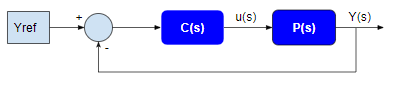
\includegraphics[width=0.8\textwidth]{exemplo_processo}
	\caption{Processo 1x1 com feedback e controlador}
	\label{img_exemplo_processo}
\end{figure}

sua função de tranferência entre a saída $Y$ e entrada $u$ será
\begin{equation}
\frac{Y(s)}{u(s)} = \frac{C(s)P(s)}{1+P(s)C(s)}
\end{equation}
sendo $C(s)$ a função do controlador.

Desta forma, caso deseje-se modelar $Y(s)$ como uma função de primeiro grau $\frac{1}{\tau s + 1}$, a equação do controlador $C(s)$ assumirá
\begin{equation}
C(s) = \frac{P^{-1}(s)}{\tau s}
\end{equation}
sendo $\tau$ o tempo de resposta do sistema, mais precisamente o tempo que o sistema leva para atingir 62,3\% do valor de seu estado estacionário.

Caso $P$ seja uma função de primeiro grau, o controlador será um PI.

Para este método de sintonia, o cálculo dos ganhos do controlador de $h_1$ desconsidera a influência de $h_2$. Tomando como base o sistema linearizado e aplicando a equação da malha fechada, o mesmo será
\begin{equation}
\overline{h_1}(s) = \frac{0,937}{s + 0,063} \overline{u_1}(s) + \frac{0,046}{s + 0,063} \overline{h_2}(s) 
\end{equation}
\begin{equation}
\overline{h_2}(s) = \frac{0,937}{s + 0,063} \overline{u_2}(s)
\end{equation}

Logo, os controladores, projetados para um tempo de resposta $\tau$ de 10 segundos, serão:
\begin{equation}
C_1(s) = C_2(s) = \frac{1}{10s} \frac{s + 0,063}{0,937} = 0,1067 + 0,0067 \frac{1}{s}
\end{equation}

\subsection{Sintonia do LQR}

O Regulador Linear Quadrático, ou LQR, é um controlador de sintonia mais simples que o PI. Seu setpoint é sempre a origem (todos os estados e entradas em zero), tornando necessárias manipulações matemáticas para controlar o sistema em outros pontos de operação. Quanto à sintonia do LQR, o controlador possui basicamente uma matriz $Q$ e uma matriz $R$, que atribuem pesos, respectivamente, aos estados e às entradas do sistema. Tomando um sistema genérico em espaço de estados:
\begin{equation}
\dot{x}(t) = A.x(t) + B.u(t)
\end{equation}
sendo $\dot{x}(t)$ as derivadas dos estados, $x(t)$ os estados, $A$ a matriz de estado, $u(t)$ as entradas e $B$ a matriz de entrada; o LQR aplicado será sintonizado de forma a minimizar a função quadrada de custo \ref{lqr_cost_func}:
\begin{equation}
J = \int_{0}^{\inf}(x'Qx + u'Ru)dt
\label{lqr_cost_func}
\end{equation} 

Segundo \cite{argentim2013}, a função de controle por feedback $u$, para o caso do LQR, é representada pela equação \ref{lqr_control_func}

\begin{equation}
u = -Kx(t)
\label{lqr_generic_control_func}
\end{equation}
sendo $K$ a matriz de ganho do feedback dos estados.

Logo, em suma, a sintonia do LQR se dá ao encontrar a matriz $K$ que minimize a função de custo \ref{lqr_cost_func}.

Para o presente caso de teste, partindo da equação \ref{espaco_estados}, tem-se como matrizes $A$ e $B$:
\begin{equation}
A = \begin{pmatrix} -0,063 & 0,046 \\ -0,063 & 0 \end{pmatrix},
B = \begin{pmatrix} 0,937 & 0 \\ 0 & 0,937 \end{pmatrix}
\end{equation}

Assumindo que nenhum estado nem entrada deve levar maior importância em relação aos outros, tem-se como matrizes de ganhos $Q$ e $R$
\begin{equation}
Q = \begin{pmatrix} 0,5 & 0 \\ 0 & 0,5 \end{pmatrix},
R = \begin{pmatrix} 0,5 & 0 \\ 0 & 0,5 \end{pmatrix}
\end{equation}

Utilizando resursos computacionais (neste caso, o comando \emph{controller\_lqr()} da biblioteca Python \emph{controlpy}, obtém-se para o sistema de teste a matriz de ganhos
\begin{equation}
K = \begin{pmatrix} 0.936 & -0,011 \\ -0,011 & 0,999 \end{pmatrix}
\end{equation}

De acordo com a equação \ref{lqr_generic_control_func}, as entradas do sistema serão então regidas pelas equações
\begin{equation}
u_1 = 0.936 {h_1}_{lqr} - 0.011 {h_2}_{lqr}
u_2 = -0.011 {h_1}_{lqr} + 0.999 {h_2}_{lqr}
\label{lqr_control_function}
\end{equation}

Porém, como o LQR traz todas as variáveis para a origem, é preciso uma translaçãonas mesmas, para que seja possível controlar o sistema em outros pontos. Desta forma, para $h_1$ e $h_2$ são feitas as seguintes operações:
\begin{equation}
{h_1}_{lqr} = h_1 - {h_1}_{sp}
{h_2}_{lqr} = h_2 - {h_2}_{sp}
\label{lqr_translation}
\end{equation}
sendo ${h_i}_{sp}$ os setpoints das alturas dos tanques no caso de teste

\section{Configuração do supervisório didático}

Como já mencionado, o programa apresentado implementa duas funções que podem ser editadas pelo usuário, de forma que seja possível uma resposta ao dispositivo conectado. O usuário pode ainda escrever suas próprias funções e alterar os objetos do código-fonte como preferir, para atender às suas necessidades. 

\subsection{Controlador PI}

Além da biblioteca \emph{python-control}, existe outra chamada \emph{simple-pid} que, como o nome indica, possui objetos que se comportam como controladores PID. Eles recebem como parâmetros seus respectivos ganhos, valores de setpoints, limites para a resposta e outros que são referenciados na página da biblioteca \href{https://pypi.org/project/simple-pid/}. Para implementá-los no programa, na função \emph{setup\_control()}, criam-se tais objetos de acordo com o código \ref{code_pi_setup}.

\begin{code}
\begin{lstlisting}
self.pids = []
self.pids.append(simple_pid.PID(0.1067, 0.0067, setpoint=2.5))
self.pids.append(simple_pid.PID(0.1067, 0.0067, setpoint=2.5))
\end{lstlisting}
\label{code_pi_setup}
\end{code}

O objeto PID da biblioteca simple-pid, quando chamado, retorna um valor numérico referente à resposta do controlador a partir de uma leitura, informada como parâmetro. Este valor pode ser escrito diretamente na porta serial, e será capturado pelo dispositivo conectado, desde que o mesmo esteja preparado para recebê-lo. No Arduino, o comando \emph{\textbf{Serial}.parseFloat()} se mostrou satisfatório.

Implementa-se, então, na função \emph{loop\_control()}, a lógica descrita acima através do código \ref{code_pi_loop}:

\begin{code}
\begin{lstlisting}
	if len(input_data) == 0:
		return

	signals = [self.pids[i](input_value) for i, input_value in enumerate(input\_data)]
	for signal in signals:
		self.porta.write('{:.2f}'.format(signal).encode('UTF-8'))
	return
\end{lstlisting}
\label{code_pi_loop}
\end{code}

O resultados podem ser conferidos na seção de resultados.

\subsection{LQR}

Uma das alternativas para a implementação do LQR no programa é a de usar a mesma biblioteca \emph{control} referenciada no Quadro \ref{qdr_used_libs}, que simula processos por funções de transferência. Nela existe a função \emph{lqr()} que retorna, entre outras saídas, a matriz de ganhos $K$ que parametriza a função de controle mostrada na equação \ref{lqr_generic_control_func}

Na função setup\_control(), escreve-se o código \ref{code_lqr_loop}, onde calcula-se primeiramente a matriz de ganhos $K$ e a armazena como uma propriedade do objeto pai. Aqui também foram definidos os desvios das variáveis (para o caso dos estados, seus setpoints), que serão empregados no cálculo do sinal de controle.

\begin{code}
\begin{lstlisting}
A = [[-0.063, 0.046],[-0.063, 0]]
B = [[0.937, 0],[0, 0.937]]
Q = [[1, 0],[0, 1]]
R = [[2, 0],[0, 2]]
K, P, V = control.lqr(A, B, Q, R)

rho = 1000
g = 9.8
k = 0.001

self.K = K
self.sp_h1 = 2.5
self.sp_h2 = 2.5
self.sp_u1 = 0
self.sp_u2 = k*math.sqrt(rho*g)

return
\end{lstlisting}
\label{code_lqr_loop}
\end{code}
Já na função loop\_control(), aplica-se a equação \ref{lqr_control_function} para o cálculo de cada sinal de controle. Porém, antes disto, realiza-se a translação nas variáveis, como mostrado na equação \ref{lqr_translation}.

Neste caso de teste, notou-se que a função \emph{Serial.parseFloat()} não foi totalmente útil, pois lia apenas a parte decimal dos valores enviados por porta serial, ignorando a parte inteira. No caso anterior, isto não se constituiu num problema, pois os sinais de controle não ultrapassaram $1 m^3/s$. Sendo assim, para o LQR, foi necessário dividir o sinal por 10, e multiplicá-lo novamente no Arduino, como constatado no código \ref{code_lqr_loop}.

Uma outra alternativa seria normalizar o sinal de controle entre 0 e 1, e desnormalizá-lo no Arduino, considerando seus limites de operação.

\begin{code}
\begin{lstlisting}
if len(input_data) == 0:
	print('No Read')
	return

input_data[0] = input_data[0] - self.sp_h1
input_data[1] = input_data[1] - self.sp_h2

signals = [-(input_data[0]*self.K[0][0] + input_data[1]*self.K[0][1]) + self.sp_u1,
		-(input_data[0]*self.K[1][0] + input_data[1]*self.K[1][1]) + self.sp_u2]
for signal in signals:
	resp = '{:.3f}'.format(float(signal)/10).encode('UTF-8')
	self.porta.write(resp)
return
\end{lstlisting}
\label{code_lqr_loop}
\end{code}

Exceto pela manipulação do sinal de controle, código utilizado no Arduino foi idêntico ao do caso do controlador PI, no anexo. Buscou-se modificá-lo o mínimo possível, pois numa aplicação real seria mais coveniente alterar as funções do supervisório, não as do controlador.

\section{Resultados}

\subsection{Controlador PI}

Com os códigos no Arduino e no supervisórios prontos, a série por via serial foi importada. Primeiramente, removeu-se as restrições de processo, para que a resposta seja mais fiel ao sistema modelado, em detrimento do sistema real. Os tanques foram partidos em $h1 = 1m$ e $h2 = 2m$.

Os resultados se encontram na Figura \ref{img_pid_sem_restricoes}.

\begin{figure}[hbt]
	\centering
	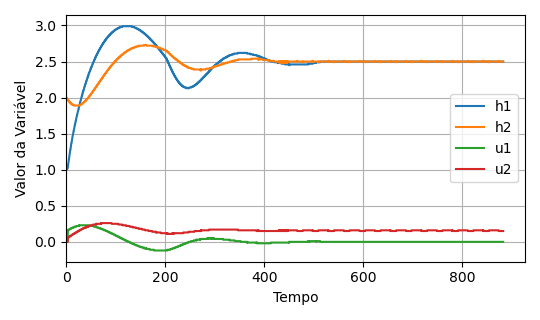
\includegraphics{PID_sem_restricoes}
	\caption{Resposta do processo para controlador PI, desconsiderando restrições de processo}
	\label{img_pid_sem_restricoes}
\end{figure}

Em seu estado estacionário, pode-se afirmar que o sistema se comporta satisfatoriamente. Como calculado na Seção \ref{comportamento_esperado}, com os setpoints de altura iguais, a bomba 1 tem estado estacionário nulo, e o sistema se mantém pela ação única da bomba 2, que assume um valor constante de $k \sqrt{\rho g{h_2}_{ss}} = 0,16$.

Como esperado, entretanto, o controle não é perfeito, pois não somente o sistema leva cerca de 10 minutos para estabilizar, como também tem comportamento dinâmico oscilatório, o que não corresponde com um sistema de primeira ordem. Porém, pelo controlador ter sido sintonizado considerando um sistema não linear, mas ter sido aplicado em outro não linear, o comportamento estacionário tem peso maior avaliação da eficiência do controle. Outro fator a ser considerado é acoplamento do sistema, que dificulta o controle preciso, já que cada controlador age somente sobre uma variável.

Apesar de nenhuma altura extrapolar o limite máximo de 4 metros, o sinal de controle assume, por vezes, valores negativos. Isto sigificaria que o fluido poderia ser retirado do tanque pelas bombas, o que não foi considerado possível neste caso. Assim, foram incluídas as seguintes restrições no processo:

\begin{enumerate}
	\item As alturas ${h_1}_{ss}$ e ${h_2}_{ss}$ devem estar compreendidas no intervalo [0, 4]m
	\item A entrada do sistema assume valores somente entre 0 e 1 $m^3/s$
\end{enumerate}

Os resultados para um sistema fisicamente mais fiel são apresentados na Figura \ref{img_pid_com_restricoes}:

\begin{figure}[!htb]
	\centering
	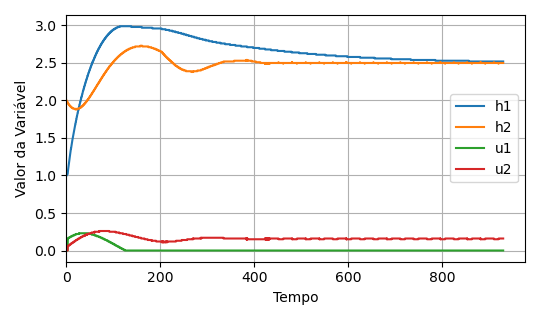
\includegraphics{PID_com_restricoes}
	\caption{Resposta do processo para controlador PI, incluindo restrições de processo}
	\label{img_pid_com_restricoes}
\end{figure}

Neste caso, para valores negativos da variável de controle, os mesmo são por sua vez substituídos por 0. Isto faz com que a altura ${h_1}_{ss}$ leve mais tempo para diminuir seu valor, pois depende somente do escoamento por gravidade e da alimentação do tanque 2, o que se reflete num tempo maior de estabilização do processo, comparado ao caso anterior.

Contudo, ainda não houve transbordamentos e os sinais de controle não atingiram valores muito altos. Assim, pode-se concluir que a estratégia do PI sintonizado em um sistema linearizado se mostrou aplicável e razoável, pois é capaz de controlar o sistema com uma boa precisão, e com pouco esforço de controle.

\subsection{LQR}

Para a resposta do sistema com o LQR, o mesmo foi iniciado com as mesmas condições iniciais do caso anterior, $h_1 = 1m$, $h_2 = 2m$. Os resultados encontram-se na Figura \ref{img_lqr_caso_1}

\begin{figure}[htb]
	\centering
	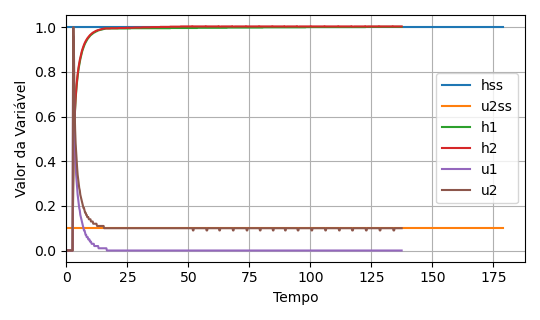
\includegraphics{LQR_caso_1}
	\caption{Resposta do LQR no primeiro caso de teste}
	\label{img_lqr_caso_1}
\end{figure}

De acordo com a resposta no tempo, assim que o controlador entra em operação, percebe-se um pico no sinal de controle, que ultrapassaria o limite estabelecido, caso não tivesse sido implementada uma salvaguarda no Arduino. A partir daí, as variáveis suavemente se aproximam do setpoint estabelecido. No geral, o sistema responde mais rapidamente que com o controlador PI do caso anterior. Porém, existe um erro estacionário maior.

De forma a suavizar o pico inicial do sinal de controle, aumentou-se os ganhos da matriz $Q$ para 2. Isto faz com que o controlador favoreça valores menores de controle, diminuindo sua eficiência, mas ganhando em um menor esforço das bombas do sistema. Como esperado e como constatado na Figura \ref{img_lqr_caso_2}, o tempo de acomodação do sistema aumenta, mas o pico não é tão grande quanto no caso 1. A eficiência do controle também é prejudicada, pois os pesos dos estados do sistema ficaram menores em relação aos pesos dos sinais de controle.

\begin{figure}[!htb]
	\centering
	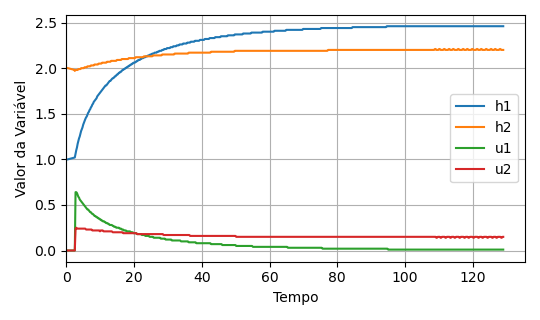
\includegraphics{LQR_caso_2}
	\caption{Resposta do LQR no caso 2}
	\label{img_lqr_caso_2}
\end{figure}

Caso se deseja-se uma melhor precisão, os pesos das matrizes de controle e de estados podem ser invertidos. O resultado disto é visto na Figura \ref{img_lqr_caso_3}.

\begin{figure}[!htb]
	\centering
	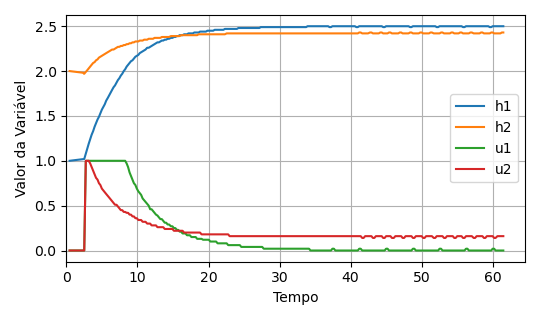
\includegraphics{LQR_caso_3}
	\caption{Resposta do LQR no caso 3}
	\label{img_lqr_caso_3}
\end{figure}

Como esperado, o sistema responde ainda mais rápido que no caso 1 e tem menor erro estacionário. A desvantagem é o pico do sinal de controle, que permanece mais tempo no limite máximo.

\section{Considerações Finais}

Neste capítulo, foram simulados e comparados dois diferentes métodos de controle num sistema de tanques acoplados. No caso do PI, apesar de haver certa demora para regular o sistema, o esforço de controle não chegou perto do limite máximo, e o estado estacionário atingido foi bem próximo dos setpoints escolhido. Em contrapartida, o LQR apresentou um erro estacionário visível, e demandou um esforço maior de controle. Por outro lado, a sintonia de ambos são diferentes, e outros valores podiam ter sido empregados para $\tau$ do sistema final modelado para o PID.

Assim como afirmado por \cite{Lourenco2007}, não existe um controlador universalmente melhor ou pior para um dado sistema. Dados os resultados atingidos, a escolha do método de controle dependeria de alguns fatores externos, como potência das bombas empregadas no sistema, tolerância de erros e tempo de resposta. Em uma aplicação industrial, o custo monetário de cada controlador e atuador certamente também seria levado em consideração. Cabe ao engenheiro responsável tomar a decisão quanto ao que seria mais vantajoso de se implemantar.

Nota-se também que o supervisório didático cumpriu seu propósito em trazer os dados em tempo real e com confiança ao usuário. Não só isso, possibilitou que os gráficos de resposta fossem facilmente armazenados e exportados em formato de imagem. Um ponto de melhoria seria permitir que o setpoint fosse modificado em tempo de execução, para que o comportamento do sistema fosse perturbado. Por outro lado, isto pode ser feito com programação Python na função do loop de controle.